\chapter{Terrain Classification for AMOS II} \label{chapter:05:terrain_classification}
Classification, one of the most widely used areas of machine learning, has a broad array of applications (see \cref{chapter:01:introduction}). To fit a classifier to a problem, one needs to define a problem data structure. Data consists of samples and discrete targets, often called classes. The samples are sooner or later converted into so called feature vectors of a fixed length. The lenght of feature vectors usually determines an input of chosen classifier and number of classes sets an output.

The classification problem in this thesis relates to AMOS II, an open-source multi sensori-motor robotic platform (see \cref{img:amosii}). The task is to classify various terrain types, while the only input comes from proprioceptive sensors. The overall process is based on simulation data and as \cref{chapter:04:neural_net_implementation} reveals, feedforward neural networks are involved.

\section{Overall Process Summary}
The very first step is to make the AMOS II simulation run (\cref{ssec:lpzrobots_sim}). Then a simple tripod gait controller is implemented (\cref{ssec:tripod_gait_controller}). To generate various terrain types, the number of variable terrain quailities and their ranges are determined (\cref{ssec:terrain_qualities}). Based on these qualities (parameters), a number of virtual terrains is defined (\cref{ssec:terrain_parameters}) and an optimality of these parameters is briefly analysed (\cref{ssec:terrains_analysis}).

Next, AMOS II (its simulation alternative) is forced to walk on every defined terrain type several times and for a sufficiently long period of time and data from all proprioceptors are saved. This data is then verified and failing experiments are removed. The data acquisition step is parameterized by a standard deviation of additive (Guassian) terrain noise and is run for several values.

Having a clean simulation data from all sensors, a feature vector structure is determined. Then a Gaussian signal noise is added. Finally, a dataset is created by splitting all the data into training, validation and testing sets. As it is indicated on \cref{img:terrain_classification_process}, several datesets and several classifiers are generated during the process. 

An optimal neural network classifier is found. The optimal network is then pruned by the algorithm developed in section X. Classification performance of developed tools are compared to a \textit{Scikit-learn} network classification library sknn [].

\begin{figure}[H]
  \centering
  \includegraphics[width=1.0\textwidth]{terrain_classification_process}
  \caption{Terrain classification process - overall diagram.}
  \label{img:terrain_classification_process}
\end{figure}

The dataset packages may differ in these parameters:
\begin{itemize}
\item terrain types included (-> number of classes)
\item sensors on input
\item samples length (number of simulation timesteps)
\item terrain noise and signal noise
\item number of samples
\end{itemize}

The trained networks may differ in following parameters:
\begin{itemize}
\item neural network structure
\item accuracy on training/validation/testing sets 
\end{itemize}

\section{Experimental Environment Specification}
Naturally, the idea of the research is to implement an online terrain classifier on the real machine. Therefore the target robot is described in the following section (\ref{ssec:amosii}).

Nevertheless, it is usually a good idea to base the reasearch on simulation data if a satisfactory simulator is available. In this case, \textit{LPZ Robots} \citep{misc:lpzrobots} is used (\cref{ssec:lpzrobots_sim}).

\subsection{Hexapod Robot AMOS II} \label{ssec:amosii}
The \textit{AMOS II} abbreviation stands for Advanced Mobility Sensor Driven-Walking Device - version II. It is a biologically inspired hardware platform of size 30x40x20 cm and weight 5.8 Kg (see \cref{img:amosii}). It is mainly used to perform experiments with neural control, memory and learning on a device with many degrees of freedom and to study the coordination of it \citep{misc:amosii}.

\begin{figure}[H]
  \centering
  \includegraphics[width=343px]{amosii}
  \caption{AMOS II. \citep{misc:amosii}}
  \label{img:amosii}
\end{figure}

In general, the robot serves as a hardware platform for neural perception-action systems experiments. The body parts are modeled on the basis of robot's biological inspiration - a cockroach.

A wide range of sensors allows AMOS II to perform several autonomous behaviours. However, only the proprioceptive sensors are important for this research, therefore, we focus on angle sensors and foot contact sensors. All of them are located on robot's legs, so the leg structure is shown on \cref{img:amosii_leg}.

\begin{figure}[H]
  \centering
  \includegraphics[width=225px]{amosii_leg}
  \caption{AMOS II. \citep{misc:amosii}}
  \label{img:amosii_leg}
\end{figure}

As figures \ref{img:amosii} and \ref{img:amosii_leg} reveal, the robot has \textbf{6 foot contact sensors} in total, one on each leg. Each of them returns a value from range $ [0.0, 1.0] $ depending on how strong the foot contact is - it is equal $ 1.0 $ if the robot stands on the leg with its full weight and it equals $ 0.0 $ when the leg is in the air.

There are three joints on each of robots legs. The thoraco-coxal (TC-) joint is responsible for forward/backward movements. The coxa-trochanteral (CTr-) joint enables elevation and depression of the leg and the last one, femur-tibia (FTi-) joint is used for extension and flexion of the tibia.

These joints are physically actuated by standard servo motors. Having the servos positions, angles of the joints are known and are also considered as propriceptive sensors. As AMOS II has six legs and there are three joints on each leg, there are \textbf{18 angle sensors} in total. There is also one backbone joint angle, however, as this one is not implemented in the simulation (see \cref{ssec:lpzrobots_sim}), it is omitted in this research.

In \cref{tab:proprioceptors} there are all the propriceptors, their shortcuts and original ranges listed. The ranges are based on the individual servos locations and are explicitly set up to avoid collisions. In \cref{sec:feature_vector_building} a normalization of these ranges is discussed.

Regarding robots actuators, the servo motors can produce variably compliant motions as if each of them were driven by a pair of agonist and antagonist muscles (see \cite{misc:amosii} for details). 

\begin{table}[H]
\centering
\caption{AMOS II - Proprioceptive sensors}
\label{tab:proprioceptors}
\begin{tabular}{|l|l|c|}
\hline
\textit{shortcut} & \multicolumn{1}{c|}{\textit{sensor description}} & \textit{original range} \\ \hline
\textbf{ATRf}         & Angle sensor, Thoraco joint, Right front leg     &                         \\ \hline
\textbf{ATRm}         & Angle sensor, Thoraco joint, Right middle leg    &                         \\ \hline
\textbf{ATRh}         & Angle sensor, Thoraco joint, Right hind leg      &                         \\ \hline
\textbf{ATLf}         & Angle sensor, Thoraco joint, Left front leg      &                         \\ \hline
\textbf{ATLm}         & Angle sensor, Thoraco joint, Left middle leg     &                         \\ \hline
\textbf{ATLh}         & Angle sensor, Thoraco joint, Left hind leg       &                         \\ \hline
\textbf{ACRf}         & Angle sensor, Coxa joint, Right front leg        &                         \\ \hline
\textbf{ACRm}         & Angle sensor, Coxa joint, Right middle leg       &                         \\ \hline
\textbf{ACRh}         & Angle sensor, Coxa joint, Right hind leg         &                         \\ \hline
\textbf{ACLf}         & Angle sensor, Coxa joint, Left front leg         &                         \\ \hline
\textbf{ACLm}         & Angle sensor, Coxa joint, Left middle leg        &                         \\ \hline
\textbf{ACLh}         & Angle sensor, Coxa joint, Left hind leg          &                         \\ \hline
\textbf{AFRf}         & Angle sensor, Femur joint, Right front leg       &                         \\ \hline
\textbf{AFRm}         & Angle sensor, Femur joint, Right middle leg      &                         \\ \hline
\textbf{AFRh}         & Angle sensor, Femur joint, Right hind leg        &                         \\ \hline
\textbf{AFLf}         & Angle sensor, Femur joint, Left front leg        &                         \\ \hline
\textbf{AFLm}         & Angle sensor, Femur joint, Left middle leg       &                         \\ \hline
\textbf{AFLh}         & Angle sensor, Femur joint, Left hind leg         &                         \\ \hline
\textbf{FRf}          & Foot contact sensor, Right front leg             & {[}0.0, 1.0{]}          \\ \hline
\textbf{FRm}          & Foot contact sensor, Right middle leg            & {[}0.0,1.0{]}           \\ \hline
\textbf{FRh}          & Foot contact sensor, Right hind leg              & {[}0.0, 1.0{]}          \\ \hline
\textbf{FLf}          & Foot contact sensor, Left front leg              & {[}0.0, 1.0{]}          \\ \hline
\textbf{FLm}          & Foot contact sensor, Left middle leg             & {[}0.0, 1.0{]}          \\ \hline
\textbf{FLh}          & Foot contact sensor, Left hind leg               & {[}0.0, 1.0{]}          \\ \hline
\end{tabular}
\end{table}

For purposes of this thesis, it is enough to know that it is possible to generate various gaits using the joints actuators and robots neural locomotion control. The gait controller used for this research is described in \cref{ssec:tripod_gait_controller}.

\subsection{LPZ Robots Simulation} \label{ssec:lpzrobots_sim}
The \textit{lpzrobots} project, developed by a research group at the University of Leipzig \citep{misc:lpzrobots} under GPL license, contains many subprojects. For purposes of this thesis, the most important ones are:

\begin{description}
\item[selforg] : homeokinetic controllers implementation framework
\item[ode\_robots] : a 3D physically correct robot simulator
\end{description}

The project is implemented in \textit{C++} and needs an Unix system to be run. It consists of two main GIT repositories to be forked - lpzrobots and go\_robots. The overall software architecture is shown on \cref{img:lpzrobots_architecture}.

\begin{figure}[H]
  \centering
  \includegraphics[width=0.5\textwidth]{lpzrobots_architecture}
  \caption{Software architecture for LPZRobots and GoRobots. \citep{misc:lpzrobots}}
  \label{img:lpzrobots_architecture}
\end{figure}

To introduce the elements in \cref{img:lpzrobots_architecture}, \textit{ThisSim} is an inherited class of another class called \textit{Simulation} and is initialized everytime the simulation is launched. It integrates all elements together, controls the environment as well as the robot and sets up initial parameters.

An instance of the \textit{Agent} class integrates all components of the agent (robot) by using the shown classes.

\begin{figure}[H]
  \centering
  \includegraphics[width=1.0\textwidth]{lpzrobots_repos}
  \caption{Structure of the two repositories (LPZRobots and GoRobots). \citep{misc:lpzrobots}}
  \label{img:lpzrobots_repos}
\end{figure}

On \cref{img:lpzrobots_repos} the cooperation of the two repositories is illustrated. With reference to \cref{app:code_documentation}, one can call the \textit{main.cpp} file from \textit{root/simulation/mbulinai22015-gorobots\_edu-fork/practices/amosii} directory as the main simulation file for purposes of the thesis. It sets up the environment with initial parameters $ controlinterval = 10 $ and $ simstepsize = 0.01 $, which means the simulation sensitivity is \textit{10 steps} per second.

It also sets the initial camera and robot position in the map. The robot position is chosen randomly and the reason for that is described in \cref{sec:data_acquisition}. The robot fixator, which is originally implemented for AMOS II is removed, so the robot starts walking right after the simulation is launched.

The \textit{main.cpp} file contains all terrain types parameters introduced in \cref{sec:virtual_terrain_types}. The required terrain to be simulated is then passed to this file as an argument. Additionally, the standard deviation value of Gaussian terrain noise (details in \cref{ssec:terrain_noise}) is set as another argument. Finally, the file is ready to take one more argument, which is a simulation noise represented by a float number. In this research it is fixed to zero though and only the terrain noise combined with a signal noise are used.

The virtual vizualization of AMOS II is illustrated on \cref{img:amosii_sim}.

\begin{figure}[H]
  \centering
  \includegraphics[width=0.8\textwidth]{amosii_sim}
  \caption{Simulation alternative for AMOS II.}
  \label{img:amosii_sim}
\end{figure}

\subsection{Tripod Gait Controller} \label{ssec:tripod_gait_controller}
The main motivation for terrain classification is to adjust current robot's gait accordingly and save some energy thereby. It is assumed that the robot is already walking, using some implemented gait, when it tries to classify the terrain. Hence, it is needed to make the simulation agent walk as well. The starting gait is decided to be the \textbf{tripod} gait.

To generate a tripod gate, a central pattern generator (CPG) is used. \citep{unpub:ai3_lec3} It is implemented as a 2-neuron neural network right inside AMOS II (\cref{img:two_neuron_network}).

\begin{figure}[H]
  \centering
  \includegraphics[width=0.5\textwidth]{two_neuron_network}
  \caption{2-neuron network oscillator. \citep{unpub:ai3_lec3}}
  \label{img:two_neuron_network}
\end{figure}

To make it work in practise, \textit{tripod\_controller.h} is written. Its initial conditions and parameters are shown in \cref{code:tripod_init}.

\begin{lstlisting}[language=C++, caption={Initialization in tripod\_controller.h}, label=code:tripod_init]
aH1 = 0; aH2 = 0;            // activities
bH1 = 0; bH2 = 0;            // biases
oH1 = 0.001; oH2 = 0.001;    // outputs
wH1H1 = 1.4; wH1H2 = 0.4;    // weights to H1
wH2H2 = 1.4; wH2H1 = -0.4;   // weights to H2
p1 = 0.35;                   // parameter for Thoraco joints
p2 = 0.3;                    // parameter for Coxa joints
\end{lstlisting}

Then, during the simulation, in \textit{tripod\_controller.h} there is a function called \textit{step()} able to control robots joints in every single simulation step. In this function three important actions come about.

\begin{enumerate}
\item \textbf{The activation function}
\begin{equation}
a_i(t+1) = \displaystyle\sum_{j=1}^{n} w_{ij}o_j(t) + b_i, i = 1, ..., n
\end{equation}

In this case, the following happen:
\begin{equation}
\begin{split}
a_{H_1} = w_{H_1,H_1} * o_{H_1} + w_{H_1,H_2} * o_{H_2} + b_{H_1} \\
a_{H_2} = w_{H_2,H_2} * o_{H_2} + w_{H_2,H_1} * o_{H_1} + b_{H_2}
\end{split}
\end{equation}

\item \textbf{The transfer function}
\begin{equation}
f(a_i) = tanh(a_i) = \frac{2}{1+e^{-2a_i}} - 1
\end{equation}

\begin{equation}
\begin{split}
o_{H_1} = tanh(a_{H_1}) \\
o_{H_2} = tanh(a_{H_2})
\end{split}
\end{equation}

\item \textbf{Joints settings}
With the reference to previous equations and variables names, the actuators are set in the sense shown on \cref{img:tripod_illustration}. The \textit{femur} joints stay with zero. This settings generates a reliable tripod gait for AMOS II.

\begin{figure}[H]
  \centering
  \includegraphics[width=250px]{tripod_illustration}
  \caption{Tripod gait controller illustration.}
  \label{img:tripod_illustration}
\end{figure}
\end{enumerate}

\section{Virtual Terrain Types} \label{sec:virtual_terrain_types}
Since the verification is based on the simulation only, the goal is to design an authentical virtual environment. For this purpose various terrain types need to be virtually imitated.

Luckily, the \textbf{LpzRobots} AMOS II simulator supports some terrain settings. In the main simulation file (\textit{main.cpp} - see \ref{app:code_documentation}), a \textit{'rough terrain'} substance is being initialized and passed through a handle to a \textit{TerrainGround} constructor.

\begin{lstlisting}[language=C++, caption={Setting a terrain ground in main.cpp}, label=code:terrain_ground]
Substance roughterrainSubstance(terrain_roughness, terrain_slip,
                       terrain_hardness, terrain_elasticity);
oodeHandle.substance = roughterrainSubstance;
TerrainGround* terrainground = new TerrainGround(oodeHandle, 
                       osgHandle.changeColor(terrain_color),
                       "rough1.ppm", "", 20, 25, terrain_height);
\end{lstlisting}

As \cref{code:terrain_ground} shows, the terrain substance is defined by four parameters: \textbf{roughness}, \textbf{slipperiness}, \textbf{hardness} and \textbf{elasticity}.

Besides the substance handle, the \textit{TerrainGround} constructor takes six more arguments.

\begin{description}
\item[terrain\_color] : simulation ground color
\item["rough1.ppm"] : an image in the .ppm format, a lowest common denominator color image file format \citep{misc:ppm}, a bitmap height file
\item[""] : texture image (not used)
\item[20] : walking area x-size 
\item[25] : walking area y-size
\item[terrain\_height] : maximum terrain height
\end{description}

\subsection{Terrain Qualities} \label{ssec:terrain_qualities}
Out of the listed ground parameters, some of them are picked up and being called \textit{terrain qualities}, as they define a specific terrain type.

It has been decided not to change the \textit{.ppm} image for various terrains and so \textit{rough1.ppm} is fixed. Also the walking area is set to (big enough) final size of \textit{20x25}. The color is variable, however, besides the simulation graphics it does not have any effect on results. 

Therefore, a virtual terrain type is defined by five qualitites. Each of them is a float number from an empirically stated range \footnote{The upper range limits have been set up based on significant changes in robot behaviour for various parameter values.}. (\cref{tab:terrain_qualities}).

\begin{table}[H]
\centering
\caption{Terrain qualities and their ranges}
\label{tab:terrain_qualities}
\begin{tabular}{lccll}
             & min value & max value \\
roughness    & 0.0       & 10.0      \\
slipperiness & 0.0       & 100.0     \\
hardness     & 0.0       & 100.0     \\
elasticity   & 0.0       & 2.0       \\
height       & 0.0       & 0.1 
\end{tabular}
\end{table}

\subsection{Terrains Parameters Determination} \label{ssec:terrain_parameters}
To determine a terrain type, one has to come up with the five parameters from \cref{tab:terrain_qualities}.

First, number of identifiable virtual terrain types needs to be determined. For purposes of this thesis, it has been decided to create \textbf{14 terrain types}. Their parameters (showed in \cref{tab:terrains_parameters}) have been set up intuitively, based on the AMOS II simulated behaviour. With respect to the qualities ranges from \cref{tab:terrain_qualities}, the values have been normed to (0, 1).

\begin{table}[H]
\centering
\caption{Virtual terrain types parameters.}
\label{tab:terrains_parameters}
\begin{tabular}{|l|l|c|c|c|c|c|}
\hline
\textit{\#}                                       & \textit{terrain title} & \multicolumn{1}{l|}{\textit{roughness}} & \multicolumn{1}{l|}{\textit{slipperiness}} & \multicolumn{1}{l|}{\textit{hardness}} & \multicolumn{1}{l|}{\textit{elasticity}} & \multicolumn{1}{l|}{\textit{height}} \\ \hline
\cellcolor[HTML]{876496}1                         & \textbf{carpet}        & 0.3                                     & 0.0                                        & 0.4                                    & 0.15                                     & 0.2                                  \\ \hline
\cellcolor[HTML]{9C9FA6}2                         & \textbf{concrete}      & 1.0                                     & 0.0                                        & 1.0                                    & 0.0                                      & 0.0                                  \\ \hline
\cellcolor[HTML]{DCE696}3                         & \textbf{foam}          & 0.5                                     & 0.0                                        & 0.0                                    & 1.0                                      & 0.7                                  \\ \hline
\cellcolor[HTML]{239614}4                         & \textbf{grass}         & 0.5                                     & 0.0                                        & 0.3                                    & 0.3                                      & 0.5                                  \\ \hline
\cellcolor[HTML]{737F9C}5                         & \textbf{gravel}        & 0.7                                     & 0.001                                      & 1.0                                    & 0.0                                      & 0.3                                  \\ \hline
\cellcolor[HTML]{D7E3FF}6                         & \textbf{ice}           & 0.0                                     & 1.0                                        & 1.0                                    & 0.0                                      & 0.0                                  \\ \hline
\cellcolor[HTML]{646464}7                         & \textbf{mud}           & 0.05                                    & 0.05                                       & 0.005                                  & 0.25                                     & 0.2                                  \\ \hline
\cellcolor[HTML]{96FABE}8                         & \textbf{plastic}       & 0.1                                     & 0.02                                       & 0.6                                    & 0.5                                      & 0.0                                  \\ \hline
\cellcolor[HTML]{6E5A3C}9                         & \textbf{rock}          & 1.0                                     & 0.0                                        & 1.0                                    & 0.0                                      & 1.0                                  \\ \hline
\cellcolor[HTML]{000000}{\color[HTML]{FFFFFF} 10} & \textbf{rubber}        & 0.8                                     & 0.0                                        & 0.8                                    & 1.0                                      & 0.0                                  \\ \hline
\cellcolor[HTML]{F2EE7C}11                        & \textbf{sand}          & 0.1                                     & 0.001                                      & 0.3                                    & 0.0                                      & 0.2                                  \\ \hline
\cellcolor[HTML]{FDB0FB}12                        & \textbf{snow}          & 0.0                                     & 0.8                                        & 0.2                                    & 0.0                                      & 0.2                                  \\ \hline
\cellcolor[HTML]{324B32}13                        & \textbf{swamp}         & 0.0                                     & 0.05                                       & 0.0                                    & 0.0                                      & 1.0                                  \\ \hline
\cellcolor[HTML]{5A4100}14                        & \textbf{wood}          & 0.6                                     & 0.0                                        & 0.8                                    & 0.1                                      & 0.2                                  \\ \hline
\end{tabular}
\end{table}

Colors linked to the terrains in \cref{tab:terrains_parameters} are used in the simulation as well as in the figures in Results section.

\subsection{Analysis of Chosen Parameters} \label{ssec:terrains_analysis}
In general, proper data preparation is an important part of classification tasks, hence a brief analysis is presented.

The goal is to imitate real terrains authentically as possible and at the same time to generate such terrains, that are clearly distinguishable from each other. The more two terrains differ the better classification results are expected.

Having five terrain qualities calls for a 5-D space, which is difficult to illustrate or even imagine. Therefore, formula \ref{eq:similarity_factor} is used to compute a similarity factor of two terrain types (the five qualities are listed in \cref{tab:terrain_qualities} and \cref{tab:terrains_parameters}).


\begin{equation} 
\label{eq:similarity_factor}
  SF_{t_1, t_2} = \displaystyle\sum_{i=1}^{5} \abs{quality(i, t_1) - quality(i, t_2)}
\end{equation} 

Naturally, equation \ref{eq:similarity_factor} ends up with $ SF_{similar} = 0.0 $ for two terrains with exactly same parameters and $ SF_{different} = 5.0 $ for two terrains differing most possibly.

The following figure (\ref{fig:terrains_parameters}) shows the variability (similarity factors) of generated terrains.

\begin{figure}[H]
  \centering
  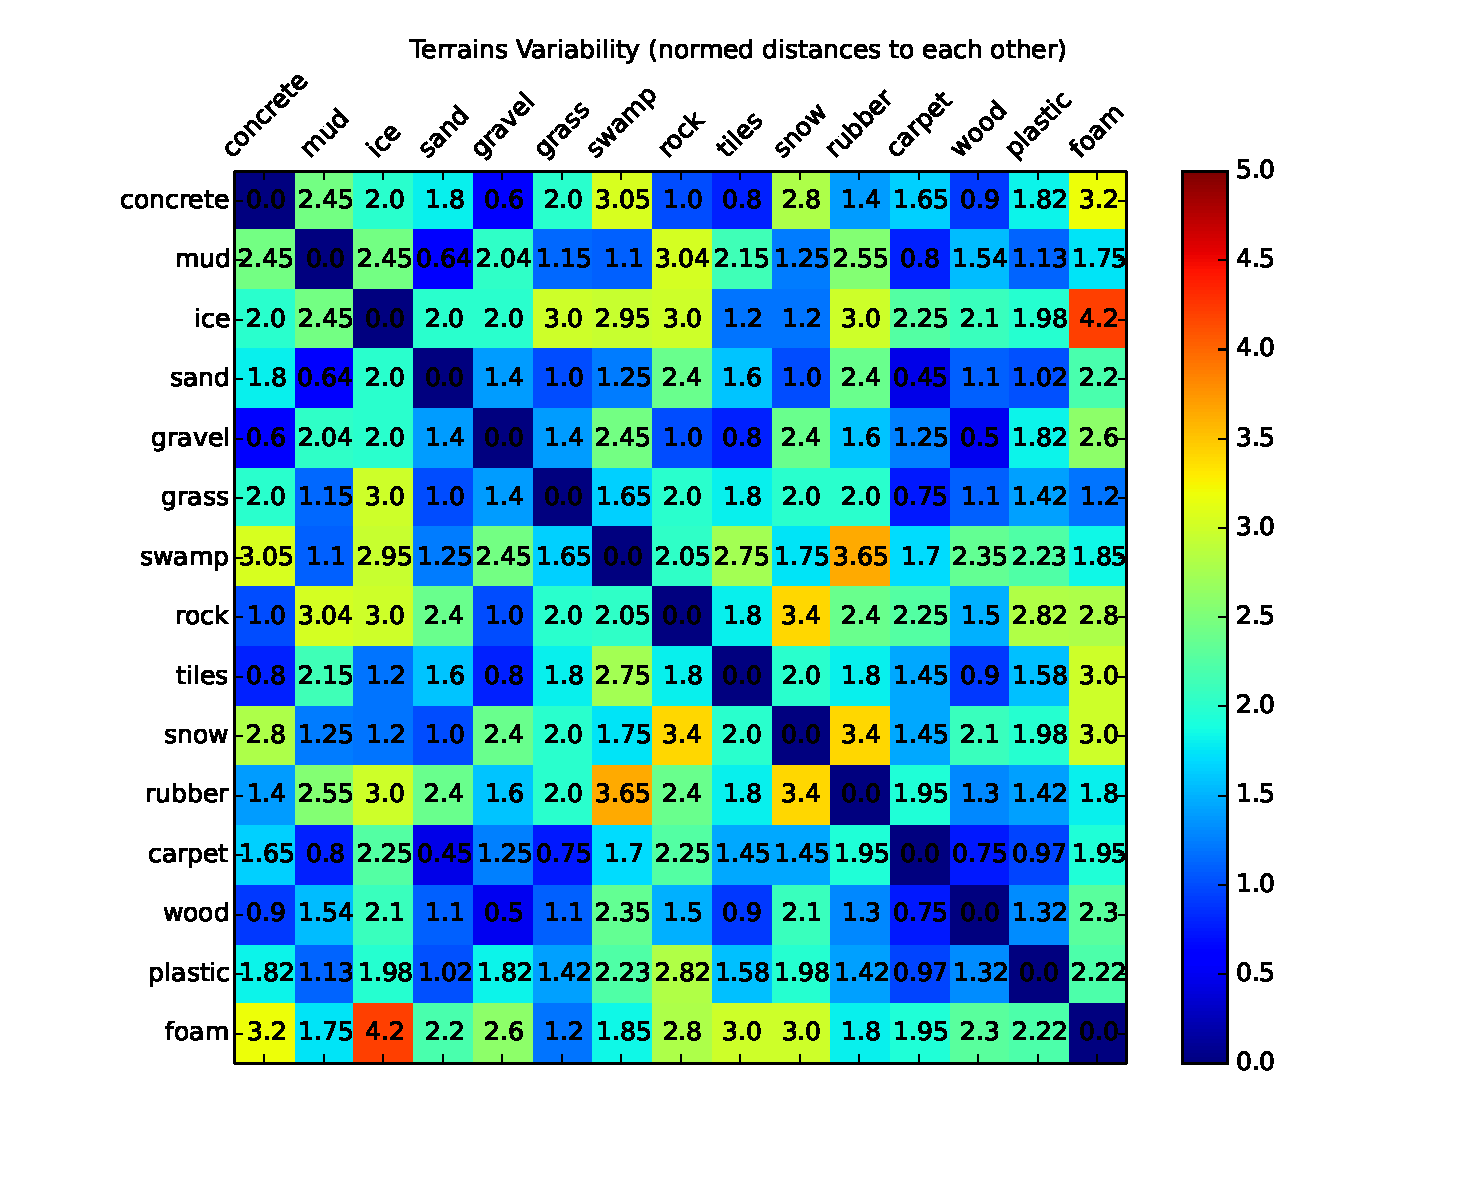
\includegraphics[width=1.0\textwidth]{terrains_variability.eps}
  \caption{Variability of generated terrain types.}
  \label{fig:terrains_parameters}
\end{figure}


\section{Feature Vector Building} \label{sec:feature_vector_building}
Determination of sensors to be used and its transformation into a feature vector

2-3 pages

\section{Data Acquisition} \label{sec:data_acquisition}
Description of how the data has been acquired from the simulation and saved as .txt, adding terrain noise

2 pages
\subsection{Terrain Noise} \label{ssec:terrain_noise}

\section{Data Processing}
Cleaning the data (deleting incomplete ones), adding signal noise, transformation into datasets, splitting into training-validation-testing sets

2-3 pages
\subsection{Signal Noise}

\section{Training and Classification}

Neural net training with several parameters and comparison with training with scikit-neuralnetwork library

2-3 pages

\subsection{Scikit-neuralnetwork library}
brief description of the library and its usage 1/2 pages

1 page